\documentclass[answers,addpoints]{exam} % answers ensures that answers are printed for each question.
% \usepackage[margin=.5in]{geometry} % 1/2 inch margins on all pages
\usepackage[utf8]{inputenc} % Define the input encoding
\usepackage[USenglish]{babel} % Define language used
\usepackage{amsmath}
\usepackage{amsfonts}
\usepackage{amssymb}
\usepackage{amsthm} % Gives us plain, definition, and remark to use in \theoremstyle{style}
\usepackage{thmtools}
\usepackage{thm-restate}
\usepackage{graphicx}

\usepackage{hyperref} % Generate hyperlinks to referenced items
\usepackage[noabbrev,nameinlink]{cleveref} % Fancy cross-references in the document everywhere
\usepackage{nameref} % Can make references by name to places
\usepackage{subcaption} % Allows for multiple figures in one Figure environment
\usepackage{siunitx} % Gives us ways to typeset units for stuff
\usepackage{csquotes} % Context-sensitive quotation facilities
\usepackage{enumitem} % Provides [noitemsep, nolistsep] for more compact lists
\usepackage{chngcntr} % Allows us to tamper with the counter a little more
\usepackage[x11names]{xcolor} % Gives access to coloring text in environments or just text, MUST be before tikz
\usepackage{ctable} % Greater control over tables and how they look
\usepackage{multirow} % Allow us to have a single cell in a table span multiple rows

\counterwithin{figure}{section}
\counterwithin{table}{section}
\counterwithin{equation}{section}

% Create a theorem environment
\theoremstyle{plain}
\newtheorem{theorem}{Theorem}[section]
% Create a numbered theorem-like environment for lemmas
\newtheorem{lemma}{Lemma}[theorem]

% Create a definition environment
\theoremstyle{definition}
\newtheorem{definition}{Defn}
\newtheorem{corollary}{Corollary}[section]
% \begin{definition}[Term] \label{def:}
%   Make sure the term is emphasized with \emph{term}.
%   This ensures that if \emph is changed, it shows up everywhere
% \end{definition}

% Create a numbered remark environment numbered based on definition
% NOTE: This version of remark MUST go inside a definition environment
\theoremstyle{remark}
\newtheorem{remark}{Remark}[definition]
%\counterwithin{definition}{subsection} % Uncomment to have definitions use section.subsection numbering

% Create an unnumbered remark environment for general use
% NOTE: This version of remark has NO restrictions on placement
\newtheorem*{remark*}{Remark}

% Create a special list that handles properties. It can be broken and restarted
\newlist{propertylist}{enumerate}{1} % {Name}{Template}{Max Depth}
% [newlistname, LevelsToApplyTo]{formatting options}
\setlist[propertylist, 1]{label=\textbf{(\roman*)}, ref=\textbf{(\roman*)}, noitemsep, nolistsep}
\crefname{propertylisti}{property}{properties}
\Crefname{propertylisti}{Property}{Properties}

% Create a special list that handles enumerate starting with lower letters. Breakable/Restartable.
\newlist{boldalphlist}{enumerate}{1} % {Name}{Template}{Max Depth}
% [newlistname, LevelsToApplyTo]{formatting options}
\setlist[boldalphlist, 1]{label=\textbf{(\alph*)}, ref=\alph*, noitemsep, nolistsep} % Set options

\newlist{nestednums}{enumerate}{6}
% [newlistname, LevelsToApplyTo]{formatting options}
\setlist[nestednums]{noitemsep, label*=\arabic*.}

% Redefine the 'end of proof' symbol to be a black square, not blank
\renewcommand\qedsymbol{$\blacksquare$} % Change proofs to have black square at end

\renewcommand{\Re}{\operatorname{Re}} % Redefine to use the command, but not the fraktur version
\renewcommand{\Im}{\operatorname{Im}} % Redefine to use the command, but not the fraktur version
% Math Operators that are useful to abstract the written math away to one spot
\DeclareMathOperator{\RealNumbers}{\mathbb{R}}
\newcommand{\TextRealNumbers}{$\RealNumbers$}
\DeclareMathOperator{\AllIntegers}{\mathbb{Z}}
\newcommand{\TextAllIntegers}{$\AllIntegers$}
\DeclareMathOperator{\PositiveInts}{\mathbb{Z}^{+}}
\newcommand{\TextPositiveInts}{$\PositiveInts$}
\DeclareMathOperator{\NegativeInts}{\mathbb{Z}^{-}}
\newcommand{\TextNegativeInts}{$\NegativeInts$}
\DeclareMathOperator{\NaturalNumbers}{\mathbb{N}}
\newcommand{\TextNaturalNumbers}{$\NaturalNumbers$}
\DeclareMathOperator{\ComplexNumbers}{\mathbb{C}}
\newcommand{\TextComplexNumbers}{$\ComplexNumbers$}
\DeclareMathOperator{\RationalNumbers}{\mathbb{Q}}
\newcommand{\TextRationalNumbers}{$\RationalNumbers$}
\DeclareMathOperator*{\argmax}{argmax} % Thin Space and subscripts are UNDER in display
\DeclareMathOperator{\Lapl}{\mathcal{L}} % Declare a Laplace symbol to be used
\DeclareMathOperator{\UnitStep}{\mathcal{U}}
\DeclareMathOperator{\sinc}{sinc} % sinc(x) = (sin(pi x)/(pi x))
\DeclareMathOperator{\XOR}{\oplus}

\newcommand{\rbpRegister}{\texttt{\%rbp}}
\newcommand{\rspRegister}{\texttt{\%rsp}}
\newcommand{\ripRegister}{\texttt{\%rip}}
\newcommand{\raxRegister}{\texttt{\%rax}}
\newcommand{\rbxRegister}{\texttt{\%rbx}}

% These packages are more specific to certain documents, but will be availabe in the template
% \usepackage{esint} % Provides us with more types of integral symbols to use
% \usepackage[outputdir=./TeX_Output]{minted} % Allow us to nicely typeset 300+ programming languages
% This document must be compiled with the -shell-escape flag if the packages above are uncommented

\graphicspath{{./Drawings/EITP20-Secure_Systems_Engineering}} % Uncomment this to use pictures in this document
% \addbibresource{./Bibliographies/CourseNum-Name.bib}

% Math Operators that are useful to abstract the written math away to one spot
% These are supposed to be document-specific mathematical operators that will make life easier
% Many fundamental operators are defined in Reference_Sheet_Preamble.tex

\begin{titlepage}
  \title{EITP20: Secure Systems Engineering --- Final Exam Study Questions \\ Lund University}
  \author{Karl Hallsby}
  \date{Last Edited: \today} % We want to inform people when this document was last edited
\end{titlepage}

\begin{document}
\pagenumbering{gobble}
\maketitle
\pagenumbering{roman} % i, ii, iii on beginning pages, that don't have content
\tableofcontents
\clearpage
\pagenumbering{arabic} % 1,2,3 on content pages

\section{Design Process}\label{sec:Design_Process}
\begin{questions}
\question{} Which are the steps involved in the overall design process of a secure system?
  \begin{solution}
    \begin{enumerate}[noitemsep]
    \item Threat Analysis
    \item Security Requirements
    \item \nameref{sec:Security_Architectures}
    \item \nameref{sec:Security_Design}
    \item \nameref{sec:Security_Evaluation}
    \end{enumerate}
  \end{solution}

  \begin{parts}
  \part{} Describe the relationship between the different steps?
    \begin{solution}
      In the Threat Analysis, the system is first scoped, to ensure that we limit our possibilities a little bit.
      Then, we attempt to find potential threats to the scoped system by performing one or more techniques (``Attacker can steal sensitive personal information.'').

      Once we find the potential threats, we use those along with any information/requirements given by the client to develop Security Requirements (``We require the use of encryption on personal data.'').

      The Security Architecture is the phase where we determine the kind of infrastructure we will need, the communication flows that are possible, find the interactions in the system, etc.
      This allows us to place our requirements onto the system as it exists already, and allow us to design for the system AND its longevity (``The personal info server is kept physically separate from others, only only communicates over mutually authenticated means using an appropriate cryptographic key.'').

      The Security Design is the process of actually choosing the standard, protocols, and hardware used to build the system (``The server will use keys generated by a Hardware Security Module, to ensure randomness.'').

      The Security Evaluation is done by going back to the Security Requirements and comparing the solutions you built in the Security Design and flows you developed in the Security Architecture to see if the requirements were satisfied.
      Other considerations can be put here too, including business ones (``Using a too difficult encryption algorithm will cause slowdowns of data requests/uses of the personal information.'').
    \end{solution}
  \end{parts}

\question{} In which way does a use-case description assist in the secure system design process?
  \begin{solution}
    It gives a general idea of \emph{how} the system will be used.
    This is important, because you can design a secure system in multiple ways to counter multiple threats.
    But, given the use-case of the client, there may be restrictions on what you can design for.
    It will help you derive the Security Requirements for the system, helping you Architect, Design, and Evaluate later in the process.
  \end{solution}

\question{} What is a threat analysis?
  \begin{solution}
    The process of finding potential threats to a system.
    These can be from inside the client's group, outside, or anywhere else.
    Using one or more methods, the applier can find current vulnerabilities, and future problems with the system.
    These are used after being given the use-case description, so that potential attack vectors can be limited to some extent.
  \end{solution}

\question{} What is the main purpose of performing a threat analysis?
  \begin{solution}
    It helps find the potential vulnerabilities in a system that \textbf{HAVE NOT} been found already.
    This will give a broader overview of the system, allowing for a more general, and hopefully, more all-encompassing secure system design.
  \end{solution}

\question{} Can you give examples of threat analysis approaches?
  \begin{solution}
    \begin{enumerate}[noitemsep]
    \item Schneier Attack Trees
    \item Microsoft's STRIDE Analysis
      \begin{enumerate}[noitemsep]
      \item Spoofing
      \item Tampering
      \item Repudiation
      \item Information Disclosure
      \item Denial of Service
      \item Elevation of Privilege
      \end{enumerate}
    \item MITRE's TARA Analysis
      \begin{enumerate}[noitemsep]
      \item Crown Jewel Analysis
      \item Cyber Risk Remediation Analysis
      \item Cyber Threat Susceptability Analysis
      \end{enumerate}
    \end{enumerate}
  \end{solution}

\question{} What is the purpose of a security requirements list?
  \begin{solution}
    To ensure that you (the secure system designer) and the stakeholders/clients/users of your system design can agree on what must be done.
    Agreement here will ensure the system is secure from both perspectives and that all parites are on the same page when it comes to the issue of security.
  \end{solution}

  \begin{parts}
  \part{} Can you list input sources for deriving security requirements?
    \begin{solution}
      \begin{itemize}[noitemsep]
      \item The use-case description.
      \item The client's system needs.
      \item The client's limitations on cost and performance.
      \item The results from the threat analysis.
      \item Further discussions and interaction between the designer and the client.
      \end{itemize}
    \end{solution}

  \part{} Which are the duties of the security engineering in the security requirements gathering process?
    \begin{solution}
      \begin{itemize}[noitemsep]
      \item To identify the threats and use them to develop the Security Requirements.
      \item To analyze the Security Requirements and correctly design to handle them.
      \item To breakdown the Security Requirements into manageable pieces that allow for simpler system design.
      \end{itemize}
    \end{solution}
  \end{parts}

\question{} Can you elaborate on the main differences between security requirements and other system requirements?
  \begin{solution}
    Security Requirements have a mixture of \emph{\textbf{BOTH}} functional and non-functional requirements.
    By having both, it can be dfficult to verify that the original requirements are fulfilled.

    Some of these requirements may be ways to ``handle'' or ``work'' with the system, such as processes, rather than properties of the system.
    A common example of this is requiring that people can only access data by giving a password, or correctly setting user permissions.

    There is always the possibility that the system may be secure now, but not in the future.
    This means that the system might not have the expected security properties, even if all the evaluations and tests indicated it did.
    This means that Security Requirements \textbf{MUST} be continually updated.
  \end{solution}

\question{} Please list at least three different “types” of security architectures?
  \begin{solution}
    The three that we discussed the most in-class and used in our reports were:
    \begin{enumerate}[noitemsep]
    \item Logical Security Architecture
    \item Physical Security Architecture
    \item Security Service Management Architecture
    \end{enumerate}
  \end{solution}

  \begin{parts}
  \part{} Explain the main differences between the different listed types?
    \begin{solution}
      Logical Security Architecture is taking the view of the \textbf{information to be secured} and designing around that.
      This involves finding the entities/actors in our system, then identifying the functions that the system must fulfill/perform.
      Next, we identify security domains/levels in the system that are in play.
      These determine where we need what kind of security and how much we trust each entity and function in each domain.

      Physical Security Architecture is done by representing the \textbf{security data model structures} and showing the ``builder's'' view of the system.
      Here, we map the security services/functions/entities identified in the logical architecture to physical security mechanisms.
      Essentially, if we specify that there is supposed to be a unique random number that acts as an ID for something, then we might say that a Hardware Security Module is required to generate those numbers.
      We do not specify any specific HSM to use, but just state that one must be used to ensure that the numbers are genuinely unique.

      Security Service Management Architecture takes a step back from designing the system for the security of the system in mind, and rather consider the maintainability of the system's security aspects.
      This is technically done at every layer of the SABSA Security Architecture model, but it is also an explicit job.
      Here, we determine how maintainable a system is given the security decisions made.
    \end{solution}
  \end{parts}

\question{} Which are the main steps preceeding the actual security design step?
  \begin{solution}
    The performance of a Security Architecture, and ensuring that the Architecture is followed when designing the system.
    Additionally, the Security Requirements make a difference on the choice of standards/protocols/hardware to use in the system.
  \end{solution}

\question{} Explain the main design choices that need to be done at the security design process.
  \begin{solution}
    \begin{itemize}[noitemsep]
    \item To find suitable security ``elements'' that can implement our chosen Secure Architecture.
    \item To find suitable security ``elements'' that can meet both our and the provided Security Requirements.
    \item To find suitable security ``elements'' that can fulfill the expected system performance and cost expectations.
    \item To make design choices that allow us to handle future, currently unknown, security weaknesses.
    \end{itemize}
  \end{solution}

\question{} What is a pen test and what is the purpose of such test?
\question{} What is a protocol analysis tool and what is the purpose of using such tool?
\question{} What is the Common Criteria (CC) standard?
  \begin{parts}
  \part{} List the 7 evaluation levels defined in CC and explain the main differences between the levels?
  \part{} List the three different system documents part of a CC and describe their main purpose.
  \end{parts}

\question{} What is CISSP?\@
\end{questions}

%%% Local Variables:
%%% mode: latex
%%% TeX-master: "../EITP20-Secure_Systems_Engineering-Study_Questions"
%%% End:


\section{Threat Analysis and Security Requirements}\label{sec:Threat_Analysis-Security_Requirements}
\begin{questions}
\question{} List three different typical security threats to an IT system?
  \begin{solution}
    \begin{enumerate}[noitemsep]
    \item Network-based threats
    \item Physical threats
    \item Software vulnerabilities
    \end{enumerate}
  \end{solution}

\question{} What is the first step in an attack tree threat analysis process?
  \begin{solution}
    There is a ``Step Zero'' that stipulates you have a \emph{good} system description.

    The first real step is to identify potential goals that the attacker could have when attcking your system as it currently exists.
  \end{solution}

\question{} Make an attack tree based analysis of a BankID system.
  \begin{solution}
    There is no single solution for this, everyone's will be different.

    For the Non-Swedes reading this, BankID is a way of verifying banking instructions and transactions through your phone as a second factor of authentication.
    To use it, you initiate some banking operation, which must be signed.
    Then, your phone will open the BankID app and ask you to input a secure 6-digit (minimum) code to ``Digitally Sign'' the transaction.
    Once done, the app closes and the trasaction is recorded and completed at the appropriate time.
  \end{solution}

\question{} List three well established threat assessment methodologies
  \begin{solution}
    \begin{enumerate}[noitemsep]
    \item Shneier Attack Trees
    \item Microsoft's STRIDE Analysis
    \item MITRE's TARA Analysis
    \end{enumerate}
  \end{solution}

\question{} Spell out the acronym STRIDE
  \begin{solution}
    \begin{description}[noitemsep]
    \item[S] Spoofing
    \item[T] Tampering
    \item[R] Repudiation
    \item[I] Information Disclosure
    \item[D] Denial of Service
    \item[E] Elevation of Privilege
    \end{description}
  \end{solution}

  \begin{parts}
  \part{} Explain the meaning of the six different concepts in STRIDE
    \begin{solution}
      \begin{description}[noitemsep]
      \item[Spoofing] Pretending to be someone or something you are not.
        Getting the correct service to communicate with someone it thinks is also the correct thing, when it really isn't.
      \item[Tampering] Modifying something (file, config, etc.) somewhere (disk, network, memory, etc.).
      \item[Repudiation] Claiming you did/didn't do something when you didn't/did.
        Essentially, the system claims you did something that you didn't do (can be honest or dishonest).
        The real question to answer here is what evidence do we have to trace this?
      \item[Information Disclosure] Providing information to someone \textbf{NOT} authorized to view it.
      \item[Denial of Service] Absorbing resources required for regular system function for malicious reasons.
      \item[Elevation of Privilege] Allowing someone to do something they should \textbf{NOT} be allowed to do.
      \end{description}
    \end{solution}

  \part{} Give examples of attacks for the six different concepts in STRIDE
    \begin{solution}
      \begin{description}[noitemsep]
      \item[Spoofing] Man-in-the-Middle.
        Impersonating the intended recipient.
      \item[Tampering] Changing an Excel Spreadsheet.
        Changing a configuration file somewhere to change the functions of the system.
      \item[Repudiation] Writing a file, then deleting the kernel log about the file requests.
      \item[Information Disclosure] Forwarding an email to someone that should not be able to see the email.
      \item[Denial of Service] Using a botnet to deny network service to some online provider.
      \item[Elevation of Privilege] You are supposed to be a regular user, but you need to elevate to administrator to run your usual programs, and IT allows people to do so.
      \end{description}
    \end{solution}
  \end{parts}

\question{} Which are the three basic steps in STRIDE?\@
  \begin{solution}
    \begin{enumerate}[noitemsep]
    \item Identify the main entities/actors in the system.
      \begin{itemize}[noitemsep]
      \item These are the people and computers that interact with the system.
      \end{itemize}
    \item Identify the main entities' interactions.
      \begin{itemize}[noitemsep]
      \item How do the people interact with the computers in the system?
      \item How do the computers interact with other computers in the system?
      \end{itemize}
    \item For each entity, perform a STRIDE analysis on each of the following items:
      \begin{description}[noitemsep]
      \item[Process] A Process is a program or set of programs that achieve or do something.
      \item[External Entity] An External Entity is one that is not \textbf{EXPLICITLY} part of \textbf{YOUR} system design.
      \item[Data Flow] A Data Flow is how information can be moved through the system.
      \item[Data Store] A Data Store is how information can be stored throughout the system.
      \end{description}
    \end{enumerate}
  \end{solution}

\question{} Which are the two main activities in a MITRE TARA security analysis
  \begin{solution}
    There is a zeroth step, the Crown Jewel Analysis for the identification of things in the system that are important to protect.
    \begin{enumerate}[noitemsep]
    \item Cyber Threat Susceptibility Analysis (CTSA)
    \item Cyber Risk Remediation Analysis (CRRA)
    \end{enumerate}
  \end{solution}

  \begin{parts}
  \part{} Which are the main input sources to these two analysis activities?
    \begin{solution}
      The question asks for 2, but I will give 3.
      \begin{enumerate}[noitemsep]
      \item Common Attack Pattern Enumeration and Classification (CAPEC)
      \item Common Weakness Enumeration (CWE)
      \item Common Vulnerabilities and Exposures (CVE)
      \end{enumerate}
    \end{solution}

  \part{} The output of these two activities are stored in special databases. What is the name of these two databases?
    \begin{solution}
      \begin{enumerate}[noitemsep]
      \item Various vulnerability and exploit databases that detail various attacks and how they can/may be executed.
        These are known as \textbf{Attack TTP Catalogs}.
      \item Countermeasure databases that explain how to mitigate the vulnerabilities and exploits that are found in the previous databases.
        These are known as \textbf{Countermeasure Catalogs}.
      \end{enumerate}
    \end{solution}
  \end{parts}

\question{} Describe briefly the different steps performed during a TARA CTSA.\@
  \begin{solution}
    \begin{enumerate}[noitemsep]
    \item Establish the Assessment Scope.
      \begin{itemize}[noitemsep]
      \item Typically this is partly done during the Crown Jewel Analysis.
      \item This is used to make sure you don't evaluate parts of the existing or new system that you are not concerned aobut.
      \end{itemize}
    \item Identify the candidate Tactics, Techniques, and Procedures (TTP).
      \begin{itemize}[noitemsep]
      \item Here, you collect \emph{\textbf{ALL}} potential TTPs that could affect your properly scoped system.
      \end{itemize}
    \item Eliminate Implausible TTPs.
      \begin{itemize}[noitemsep]
      \item If you perform Step 2 correctly, you will have WAY too many TTPs to mitigate for you system to ever work.
      \item You must use your best judgment to remove the ones that are implausible to occur in your system.
      \end{itemize}
    \item Apply some scoring model.
      \begin{itemize}[noitemsep]
      \item MITRE has a scoring model provided that can be quite useful.
      \item These will be the scores that you use in the Threat Matrix to find the best TTPs to design against.
      \end{itemize}
    \item Construct a Threat Matrix.
      \begin{itemize}[noitemsep]
      \item The scores used in the Threat Matrix are based off the scoring model that is created in the previous step.
      \item This will show you the which TTPs that remain are the most important to design against.
      \end{itemize}
    \end{enumerate}
  \end{solution}

  \begin{parts}
  \part{} What does CAPEC contain and how it is used in a TARA analysis?
  \part{} What does CWE contain and how it is used in a TARA analysis?
  \part{} What does CVE contain and how it is used in a TARA analysis?
  \end{parts}

\question{} Describe briefly the different steps performed during a TARA CRRA
\question{} Where can one find TTP mitigation solutions?
\question{} Which are the four different mitigation types?
\question{} Which are the steps used to obtain a final ranking table for countermeasures?
\question{} How do one select final TARA recommendations based on a countermeasure ranking table?
\question{} Which are the three mandatory parts of a TARA TTP recommendation?
\question{} Which are the different input sources to the security requirements derivation process?
\question{} Which are the main outputs from the attack tree, the STRIDE and the TARA process respectively which are used to derive high-level security requirements?
\question{} Give example of high level security requirements for a Bank ID system
\question{} Give example of low level security requirements  for a Bank ID system
\question{} Describe a four step approach for security requirements identification and documentation
\end{questions}

%%% Local Variables:
%%% mode: latex
%%% TeX-master: "../EITP20-Secure_Systems_Engineering-Study_Questions"
%%% End:


\section{Security Architectures}\label{sec:Security_Architectures}
\begin{questions}
\question{} Describe what constitutes a security architecture and give some examples.
  \begin{solution}
    A Security Architecture has graphical and textual representations of a security system.
    It includes relations, trust levels, trust relationships, and interfaces between different parts of the system.
    It also has security and system boundaries to delimit different parts of the system that have various properties.
  \end{solution}

\question{} The Sherwood Applied Business Security Architecture (SABSA) consist of 5 layers and one cross layer.
  \begin{parts}
  \part{} Describe the different layer views and list the names of the different layers.
    \begin{solution}
      \begin{enumerate}[noitemsep]
      \item Contextual Security Architecture is the view the business has of the system.
        It is quite similar to the Security Requirements.
      \item Conceptual Security Architecture is the highest-level view that an engineer can have of the system.
        This includes the general breakdown into secure portions of a system.
      \item Logical Security Architecture is the next level, that deals with data and its logical flows.
        Here, the way that data and its logical propagation are safeguarded is first developed.
      \item Physical Security Architecture is the 3rd design level.
        Here, the specific high-level security requirements and previous security architecture levels are combined to choose what needs to be done to secure the data.
      \item Component Security Architecture is the lowest level of the SABSA Security Architecture.
        Here, the actual protocols, standards, and hardware are chosen.
      \item Security Service Management Architecture is the ``cross layer''.
        It is concerned with how to maintain the system and its security.
      \end{enumerate}
    \end{solution}

  \part{} Give examples of questions the different SABSA architecture views are supposed to answer.
    \begin{solution}
      \begin{enumerate}[noitemsep]
      \item Contextual Security Architecture
        \begin{itemize}[noitemsep]
        \item What does the business need from the system?
        \item Why do we need to mitigate against these risks and threats?
        \item How do we protect the processes in this system?
        \item Who are going to be the ones using the system?
        \item Where is this system going to be geographically located and where is this product going to be used?
        \item When does the client require this system and for how long?
        \end{itemize}
      \item Conceptual Security Architecture
        \begin{itemize}[noitemsep]
        \item What does the client need to have protected?
        \item Why are these risks that need to be mitigated and do these assets need protection?
        \item How do we provide protection, in very high-level technical and maanagement security terms/strategies?
        \item Who are the people/organizations involved in the security management and the assumed trust relationships?
        \item Where is protection needed in terms of security domains?
        \item When is the relevant time scope(s) of the system's protection?
        \end{itemize}
      \item Logical Security Architecture
        \begin{itemize}[noitemsep]
        \item What is the actual information being secured?
        \item Why shall this security policy be applied to the system?
        \item How are the actual security services in the system put together?
        \item Who are the entities in the system and how can they interact?
        \item Where are the security domains and the relationships between the domains?
        \item When is the security processing cycle?
        \end{itemize}
      \item Physical Security Architecture
        \begin{itemize}[noitemsep]
        \item What is the data model and security-related data structures?
        \item Why are these the rules that drive logical decisions in the system?
        \item How do these security mechanisms work to provice security and what physical machines or modules are needed?
        \item Who are the users, the applications they use, and the security interface?
        \item Where is the required security infrastructure required to provide the security?
        \item When is the dependency in the system present in the form of execution control structures?
        \end{itemize}
      \item Component Security Architecture
        \begin{itemize}[noitemsep]
        \item What are the data field specifications, address specifications, etc.
        \item Why are we using these security standards and best practices?
        \item How are the entities/modules, tools, etc.\ used and put together?
        \item Who are the users' identities, privileges, functions, actions, Access Control Lists?
        \item Where are the computing processes, nodes addresses, and inter-process protocols?
        \item When are the security step timings and sequencing?
        \end{itemize}
      \item Security Service Management Architecture
        \begin{itemize}[noitemsep]
        \item What is the operational continuity and information processing of the system?
        \item Why do we need to minimize operational risks and mitigate failures/disruptions?
        \item How do we perform these specialized security-related operations?
        \item Who do we support? All users and their applications?
        \item Where do we perform maintainance from and on?
        \item When do we schedule things and execute our time-table of security-related operations?
        \end{itemize}
      \end{enumerate}
    \end{solution}
  \end{parts}

\question{} Which are the three different types of security services in a logical security architecture?
  \begin{solution}
    \begin{enumerate}[noitemsep]
    \item Prevention services
    \item Detection, Notification, Assurance, and Event Collection services
    \item Recovery and Restoration services
    \end{enumerate}
  \end{solution}

  \begin{parts}
  \part{} List and explain examples of services part of the non-prevention type of security services.
    \begin{solution}
      \begin{itemize}[noitemsep]
      \item Detection, Notification, Assurance, and Event Collection services
        \begin{itemize}[noitemsep]
        \item Log review
        \item Message integrity verification
        \item Security monitoring
        \item Audit trails
        \item Security Training/awareness
        \item Intrusion Detection
        \end{itemize}
      \item Recovery and Restoration services
        \begin{itemize}[noitemsep]
        \item Incident response
        \item Data replication
        \item Data backup
        \item Disaster recovery
        \item Crisis management
        \end{itemize}
      \end{itemize}
    \end{solution}
  \end{parts}

\question{} Describe each of the different prevention security services in more details.
  \begin{parts}
  \part{} Give example of at least four different Entity Security Services and how they contribute to security prevention.
    \begin{solution}
      \begin{enumerate}[noitemsep]
      \item Unique Entity naming
      \item Entity registration
      \item Entity credentials certifications
      \item Directory services
      \item Entity authorization
      \item User authentication
      \item Device authentication
      \end{enumerate}
    \end{solution}

  \part{} Give example of at least four different Communication Security Services and how they contribute to security prevention.
    \begin{solution}
      \begin{enumerate}[noitemsep]
      \item Session authentication
      \item Message origin authentication
      \item Non-repudiation
      \item Message reply protection
      \item Traffic flow confidentiality
      \item Security administration
      \item User support
      \item Physical security services
      \item Environmental security services
      \end{enumerate}
    \end{solution}

  \part{} Give example of at least four different Application-level Security Services and how they contribute to security prevention.
    \begin{solution}
      \begin{enumerate}[noitemsep]
      \item Entity authorization
      \item Logical access control
      \item Audit trails
      \item Stored data integrity protection
      \item Stored data confidentiality
      \item Software integrity protection
      \item Software licensing management
      \item System config protection
      \item Data replication
      \item Data backups
      \item Software replication
      \item Software backups
      \item Trusted time
      \item Secure user interface
      \end{enumerate}
    \end{solution}

  \part{} Give example of at least four Security Management Services and how they contribute to security prevention.
    \begin{solution}
      \begin{enumerate}[noitemsep]
      \item Security policy management
      \item Security training and awareness
      \item Security ops management
      \item Security provisioning
      \item Security monitoring
      \item Security measurements and metrics
      \item Security administration
      \item User support
      \item Physical security devices
      \item Environmental security services
      \end{enumerate}
    \end{solution}
  \end{parts}

\question{} Draw a picture showing the relations between major different security services from a systems point of view.
  \begin{solution}
    \includegraphics[scale=0.5]{./Drawings/EITP20-Secure_Systems_Engineering/Major_Security_Services_Relations.png}
  \end{solution}

\question{} A logical security architecture can be created using a six steps methodology:
  \begin{parts}
  \part{} Describe each of the different steps
    \begin{solution}
      \begin{enumerate}[noitemsep]
      \item Identify the main entities.
        Here, the users and the physical components in the system(s) are identified.
        Who is doing something and what is executing the user's actions?
      \item Identify the major functions in the system.
        Each computing entity has some function(s) that it needs to fulfill.
        What does each hardware entity need to do?
      \item Identify the security domains and their associations.
        Each entity and function exists within a security domain, i.e.\ how much they are trusted.
        In addition, how do these security domains interact with each other?
      \item Identify security services already meeting the Security Requirements.
        There may be some properties of the system that already meets the requirements as laid out in the Security Requirements.
        Identify these.
        There may also be security services that are required to meed the Security Requirements, identify these too.
      \item Map security services to the functional entities.
        Take the security services from the previous step, and match them together with the entities in the system.
      \item Create a graphical view of the logical architecture.
        It is easier to see how these security services get mapped to the entities and security domains if it is done in a graphical view and their interactions are shown.
        Each computing entity should be a box, each flow of communication an arrow, each user shown, and the computers/users should be grouped together into their security domains.
      \end{enumerate}
    \end{solution}

  \part{} What is the end result?
    \begin{solution}
      A general logical view of the system to see what data needs to be secured and how that should be done.
      This will also specify the security services that should be used, the security domains, the users, the computing entities, among others.
    \end{solution}

  \part{} Give an example of a logical security architecture.
    \begin{solution}
      See Slides 25--31 of Lecture 3.
    \end{solution}
  \end{parts}

\question{} What is a Physical Security Architecture?
  \begin{solution}
    A Physical Security Architecture is the general specification of how to implement the security given by the Logical Security Architecture.
    The expected outcome is a specification of the security solutions offered in the system, including the platform, software, and hardware security functions.
  \end{solution}

\question{} A physical security architecture when using the SABSA includes making a mapping to physical security mechanisms.
  \begin{parts}
  \part{} Describe what is meant by a ``User interface and naming'' mechanism and give examples
  \part{} Describe what is meant by a ``Authorization and access control'' mechanism and give examples
  \part{} Describe what is meant by a ``Monitoring and incident'' mechanism and give examples
  \part{} Describe what is meant by a ``Naming and Registration'' mechanism and give examples.
    \begin{solution}
      The Naming and Registration mechanism is concerned with how we identify the entities within our system.
      Additionally, when they have been given an identifier to recognize by, how we can register them with a system to ensure that when an entity claims to be something with a certain name, we can verify that.

      This typically includes:
      \begin{itemize}[noitemsep]
      \item Unique Naming
        \begin{itemize}[noitemsep]
        \item Using a common naming standard.
        \item Using a common naming procedure.
        \item Using a directory system to separate different names.
        \end{itemize}
      \item Entity Registration
        \begin{itemize}[noitemsep]
        \item Using a standard registration policy.
        \item Having a standard registration procedure.
        \item Using a registration authority system.
        \end{itemize}
      \item Public Key Certification
      \item Directory Services
        \begin{itemize}[noitemsep]
        \item Having a directory system.
        \item Having a directory access protocol.
        \item Having a directory object and attribute syntax rules.
        \item Allowing for directory replication.
        \end{itemize}
      \end{itemize}
    \end{solution}

  \part{} Describe what is meant by a ``Storage and Runtime'' mechanism and give examples.
    \begin{solution}
      This is concerned with how we store data securely and use it securely during runtime.
      \begin{itemize}[noitemsep]
      \item Data confidentiality
      \item Data integrity
      \item Software integrity
      \item Secure Execution
        \begin{itemize}[noitemsep]
        \item Secure hardware modules
        \item Secure execution enclaves
        \item Secure virtual machines
        \item Protected execution
        \end{itemize}
      \item Software licensing Protection
      \item Data and software replication
      \end{itemize}
    \end{solution}

  \part{} Describe what is meant by a ``Physical Security'' mechanism and give examples.
    \begin{solution}
      This is concerned with the physical security of a location.
      \begin{itemize}[noitemsep]
      \item Physical Security
        \begin{itemize}[noitemsep]
        \item Locks on doors
        \item Locked server rooms
        \item Physical protection of cables
        \item Personnel identification
        \end{itemize}
      \item Environmental Security
      \item Personnel Security
        \begin{itemize}[noitemsep]
        \item Background checks
        \item Vetting procedures
        \item Training Courses
        \end{itemize}
      \end{itemize}
    \end{solution}

  \part{} Describe what is meant by an ``Authentication and Session'' protection mechanism and give examples.
    \begin{solution}
      When a registered name wants to access our system, how do we ensure that they are who they say they are and make sure that they have not been compromised?
      \begin{itemize}[noitemsep]
      \item Entity Authentication
        \begin{itemize}[noitemsep]
        \item Login procedure
        \item User passwords/tokens
        \item Authentication protocol
        \end{itemize}
      \item Session Authentication
      \item Message Integrity
        \begin{itemize}[noitemsep]
        \item Message Authentication Codes (MACs)
        \item Hashing
        \end{itemize}
      \item Message Confidentiality
      \item Message Reply Protection
      \item Non-repudiation
      \end{itemize}
    \end{solution}

  \end{parts}

\item What must in addition to the security mechanisms be specified in the physical security architecture?
\item Give example of platform security solution that can be used to build solutions meeting a logical security services and can be used to protect the chosen physical security mechanism?
\item For the SSO logical security architecture given at the lecture, perform the following:
  \begin{parts}
  \part{} Identify the main physical security mechanisms needed in the corresponding physical security architecture.
  \part{} Identify the main platform security components needed to fulfil the architecture
    \begin{subparts}
    \subpart{} Suggest concrete platform security mechanisms to use for the physical realization.
    \end{subparts}
  \end{parts}
\end{questions}

%%% Local Variables:
%%% mode: latex
%%% TeX-master: "../EITP20-Secure_Systems_Engineering-Study_Questions"
%%% End:


\section{Security Design}\label{sec:Security_Design}
\begin{itemize}
\item Can you list four different principles upon which a security design should be based?
  \begin{itemize}[noitemsep]
  \item Give a motivation for each of the listed design principles
  \end{itemize}

\item Describe the process steps to perform when going from a security architecture to a design specification
\item What is typical the role of unique identities in security systems?
  \begin{itemize}[noitemsep]
  \item Give example of three different widely used identity types?
  \end{itemize}

\item What is the problem from privacy perspective with using fixed identities?
  \begin{itemize}[noitemsep]
  \item \item Describe two different methods for avoiding the identity privacy problem in a system design
  \end{itemize}

\item What is a digital certificate and how it is used?
  \begin{itemize}[noitemsep]
  \item \item Which are the most important data fields in an X.509 certificate?
  \end{itemize}

\item Which is the far most used authentication principle over http?
  \begin{itemize}[noitemsep]
  \item Describe the different steps in an HTTP basic authentication
  \item Under which circumstances can basic authentication be used
  \item How are typically basic authentication treated at the server side and what is the main reason for using this type of storage?
  \end{itemize}

\item Describe the principles behind hardware token based authentication
\item What is the rationale behind two factor authentication?
\item What are the main differences between:
  \begin{itemize}[noitemsep]
  \item TLS server authentication
  \item TLS client certificate authentication
  \item TLS pre-share key authentication
  \end{itemize}

\item Explain the main principle behind an object security scheme
  \begin{itemize}[noitemsep]
  \item How does it differs from a session protection scheme like TLS or IPsec?
  \end{itemize}

\item What does RBAC and ABAC stand for with respect to access control systems?
  \begin{itemize}[noitemsep]
  \item Explain the main differences between RBAC and ABAC
  \end{itemize}

\item What is the purpose with an access token?
  \begin{itemize}[noitemsep]
  \item What does a SAML assertion contain?
  \end{itemize}

\item How can a Hardware Security Module (HSM) assist in protection of cloud data storage?
\item List a couple of widely used commercial server anti-virus tools
\item How can the security of a Docker container be enhanced beyond using default configurations?
\item How can a Web design be made to make ``clickjacking'' less likely?
\item What is the main difference between key provisioning of a public key system compare to a symmetric key-based systems?
  \begin{itemize}[noitemsep]
  \item What are the key issues to consider when making a public key issuing design?
  \item Which are the key issues to consider when making a symmetric key issuing design?
  \end{itemize}

\item List the three main different intrusion detection principles and explain how they work on high level
\item What is syslog and how is it typically used?
\item What is the main risks with a debug interface (like JTAG) and how should it be treated in a product design to avoid these risks?
\item Which are the three different most severe attacks threats against smart card designs and which are the typical countermeasures?
\item Give three examples of widely used NIST security standards and what they specify?
\item What does IETF stand for?
  \begin{itemize}[noitemsep]
  \item Give example of two well-knows IETF security standards and explain what they specify?
  \end{itemize}

\item Which type of security standards are done by IEEE and 3GPP respectively?
\item What is the difference between public industry bodies and industry standards?
\item What is meant by a cancellable biometric protection scheme?
  \begin{itemize}[noitemsep]
  \item Describe how to achieve a cancellable biometric matching system
  \item Which alternative biometrics protection approaches can be used?
  \end{itemize}
\end{itemize}

%%% Local Variables:
%%% mode: latex
%%% TeX-master: "../EITP20-Secure_Systems_Engineering-Study_Questions"
%%% End:


\section{Security Evaluation}\label{sec:Security_Evaluation}
\begin{questions}
\question{} What is the purpose with a security review and when should it be performed?
  \begin{solution}
    A security review is intended to perform a general ``sanity'' check that the chosen Security Architecture makes sense.
    It also helps identify potential gaps in the Security Architecture that might have been missed.
    It can also provide a business evaluation of the chosen architecture to find business consequences.
    Lastly, we take the perspective of an attacker attempting to break into the system.

    Generally, this is done after the Architecture and Design is completed, but performing it regularly during these steps also works.
  \end{solution}

\question{} At which four main levels do you typically perform a security evaluation?
  \begin{solution}
    \begin{enumerate}[noitemsep]
    \item Security Architecture Review
    \item Design against Requirements Review
    \item Design Review
    \item Implementation Review
    \end{enumerate}
  \end{solution}

  \begin{parts}
  \part{} At which occasion should they be done?
    \begin{solution}
      \begin{enumerate}[noitemsep]
      \item After the Security Architecture design selections.
      \item Before the Security Design Specification.
      \item After the Security Design Specification.
      \item Before the system's release.
      \end{enumerate}
    \end{solution}
  \end{parts}

\question{} Mention three different aspects to consider at an architecture ``sanity check'' review.
  \begin{solution}
    \begin{enumerate}[noitemsep]
    \item System purpose vs. Security
    \item Usability Check
    \item Administrative Burden
    \end{enumerate}
  \end{solution}

  \begin{parts}
  \part{} For each aspect, list what should be considered?
    \begin{solution}
      \begin{enumerate}[noitemsep]
      \item
        \begin{itemize}[noitemsep]
        \item Does the chosen Security Architecture change any system functions?
        \item Are the security functions adding any new system properties?
        \item Can these new security functions be accepted the end-users?
        \end{itemize}
      \item
        \begin{itemize}[noitemsep]
        \item Will the security functions have any direct usability considerations?
        \item If they do, are they acceptable?
        \item Is it possible to modify the system to make it easier to use while maintaining security?
        \end{itemize}
      \item
        \begin{itemize}[noitemsep]
        \item Which routines and security policies are necessary to make the architecture functional?
        \item How costly is it to maintain the routines and policies?
        \item How much will the system be dependent on manual routines?
        \end{itemize}
      \end{enumerate}
    \end{solution}
  \end{parts}

\question{} Mention three different aspects to consider at an architecture business review.
  \begin{solution}
    \begin{enumerate}[noitemsep]
    \item Security Control
    \item Customer Relations
    \item Business Risks and Opportunities
    \end{enumerate}
  \end{solution}

  \begin{parts}
  \part{} For each aspect, list what should be considered?
    \begin{solution}
      \begin{enumerate}[noitemsep]
      \item
        \begin{itemize}[noitemsep]
        \item Who is in control of the system's security funcctions?
        \item Will the security control give the party controlling these an advantage?
        \item If so, make sure the security controls are kept within the business' domains.
        \end{itemize}
      \item
        \begin{itemize}[noitemsep]
        \item Will the suggested Security Architecture influence any existing or future customer relations?
        \item If so, this \emph{\textbf{MUST}} be highlighted and discussed with the client.
        \end{itemize}
      \item
        \begin{itemize}[noitemsep]
        \item Will the architecture influence the current business in a direct or indirect way?
        \item If so, can we make sure the business implications are favorable?
        \end{itemize}
      \end{enumerate}
    \end{solution}
  \end{parts}

\question{} What do you perform during a security requirements review?
  \begin{solution}
    The Security Requirements are revisted to ensure the current System Architecture addresses \textbf{ALL} the mandator requirements.
    Any that are missing are added and the Security Design is updated to reflect this.
  \end{solution}

\question{} Mention four different aspects to consider at a design review.
  \begin{solution}
    \begin{enumerate}[noitemsep]
    \item Standards Review
    \item Data Representation
    \item Protocols
    \item Review of New Designs
    \end{enumerate}
  \end{solution}

  \begin{parts}
  \part{} For each aspect, list what should be considered?
    \begin{solution}
      \begin{enumerate}[noitemsep]
      \item
        \begin{itemize}[noitemsep]
        \item Are standards used when possible?
        \item Are the chosen standards appropriate for this use-case?
        \item Are our own design choices compliant with the relevant standards?
        \end{itemize}
      \item
        \begin{itemize}[noitemsep]
        \item Is the data format used appropriate for the system's functions?
        \item Is the data representation in a protected format when needed?
        \item Is the data accessible whenever it is needed?
        \item Is the footprint required for securing this data acceptable?
        \end{itemize}
      \item
        \begin{itemize}[noitemsep]
        \item Are all new protocol designs evaluated and verified?
        \item Are the protocol's performance figures acceptable?
        \end{itemize}
      \item
        \begin{itemize}[noitemsep]
        \item In the new designs, do the parts have security soundness?
        \item Is ti possible to verify (theoretically or formally) any new design choices?
        \item Is the performance of these new design choices acceptable?
        \item Has the new design been reviewed by independent experts?
        \end{itemize}
      \end{enumerate}
    \end{solution}
  \end{parts}

\question{} Describe a process for issuing and security testing of a software product
  \begin{parts}
  \part{} What is the role in the process for the security officer, the security architect, the security master and security penetration tester respectively?
  \end{parts}

\question{} Give examples of things to consider during a performance review of a design?

\question{} What is the purpose of trying to ``measure'' the security of a design?
\question{} A simple security measurement takes three basic security characteristics into account:
  \begin{parts}
  \part{} Which three characteristics are then measured and how to you combine the measurements to get an overall measurement of a system?
  \end{parts}

\question{} Consider the smart card security system in \Cref{fig:Smart_Card_Security_System}.
  Assume the side-channel and physical channel break are equal important and the overall smart card security is the minmum strength of the two nodes.
  Calculate the smart card security score using the weighted weakest link approach.
  \begin{figure}[h!]
    \centering
    \includegraphics[scale=0.35]{./Drawings/EITP20-Secure_Systems_Engineering/Smart_Card_Security_System.png}
    \caption{Smart Card Security System}
    \label{fig:Smart_Card_Security_System}
  \end{figure}


\question{} How can the sensitivity for a certain security component be calculated?
\question{} What is a CVE database? Which organizations maintain global CVEs?
\question{} Which are the tree basic categories for which CVE scoring is based
  \begin{parts}
  \part{} Briefly explain each of the three categories and which security aspects are considered for each of them?
  \end{parts}

\question{} A communication product have three different categories of weaknesses, buffer overflow, TPM weaknesses, and authentication weakness with the CVE list below. Calculate an overall vulnerability score for the product (use the NIST CVE database to obtain the individual scores).
  \begin{parts}
  \part{} Buffer overflow: CVE--2019--2304, CVE--2019--2242, CVE--2019--10572
  \part{} TPM:\@ CVE--2019--16863, CVE--2018--6622
  \part{} Authentication: CVE--2019--3768, CVE--2019--5108,CVE--2019--17627, CVE--2018--5389
  \end{parts}

\question{} Explain the terms TOI, PP, ST and EAL used in CC evaluations.
\question{} What is the purpose with the PPs?
\question{} What is the main differences between the different EAL levels?
\end{questions}

%%% Local Variables:
%%% mode: latex
%%% TeX-master: "../EITP20-Secure_Systems_Engineering-Study_Questions"
%%% End:


\section{Protocol Analysis}\label{sec:Protocol_Analysis}
\begin{itemize}
\item What is mutual authentication?
\item Which attacks are typically applicable to an authentication protocol?
\item What is a man-in-the-middle attack? How could you prevent it?
\item What is a replay attack? How could you prevent it?
\item What is a reflection attack? How could you prevent it?
\item What is a labeled multiset rewriting rule? What are $l$, $r$, $a$?
\item What is a state agent fact $St\_R\_s(A, id, \ldots)$ ?
\item What are In and Out facts? What are Send and Recv action facts? When do you have them?
\item What is a protocol rule? What is an action fact?
\item What is fresh rule? What is $Fr()$ fact?
\item What is infrastructure rule? How do you write the key generation for PKI? How can you generate private/public keys and publish public keys using Fr, Ltk, Out, PK facts?
\item What is an initialization rule? How do you write the initialization rule for a given protocol (e.g. a public key-based protocol)? What is Create action fact?
\item What is the meaning of well-formedness? How could you write protocol rules that are well-formed?
\item How can you write protocol rules for a given protocol?
\item Assume that you are given a public key-based protocol. How could you write the initialization and protocol rules for it? How could you prepare the protocol and split the roles?
\item What is protocol instrumentation? What is a claim event $Claim\_claimtype(A,t)$?
\item What is secrecy?
\item How is the role instrumentation for secrecy? What is $Claim\_secret(A,M)$? Where do you place the hexagon for secret (M) in role instrumentation for secrecy?
\item What is a compromised agent? When an agent is honest? What are Honest and Rev action facts?
\item How can you verify if secrecy claims hold for a given protocol? (See examples in slides 31--34 of lecture 9. See also an exercise here).
\item What is forward secrecy?
\item How can you find out that a given protocol provides forward secrecy? (See examples in slides 36--37 of lecture 9).
\item How is the role instrumentation for authentication? What are $Claim\_commit$ and $Claim\_running$ events? Where do you place Commit and Running hexagons when A wants to agree with B?\@ Where do you place them when B wants to agree with A?\@
\item How do you model a protocol using Tamarin? How do you write a labeled multiset-rewriting rule in Tamarin?
\item What are linear and persistent facts in Tamarin? When do you use ! or \textasciitilde{} or \$ in Tamarin?
\item What does $\langle x, y \rangle$ mean in Tamarin?
\end{itemize}
%%% Local Variables:
%%% mode: latex
%%% TeX-master: "../EITP20-Secure_Systems_Engineering-Study_Questions"
%%% End:


\end{document}